\subsubsection{Application Programming Interfaces (APIs)}
\label{sec:APIs}

Aufbauend auf dem abgeschlossen Administrationsbereich, werden im Nachfolgenden Verlauf Application Programming Interfaces, kurz APIs, implementiert. Aufgabe solcher APIs ist es Informationen in maschinenleserlicher Form für andere Teilbereiche des Systems bereitzustellen. Die dargestellten Informationen werden von den aufrufenden Systemen genutzt, um Inhalte dynamisch darzustellen. Als Beispiel wird der vorgestellte Prototyp die Menge der benachbarten Panoramas über eine solche API beziehen und darauf aufbauend dem Benutzer die Navigationspfeile entsprechend präsentieren. Die Implementierung einer API wird im folgenden an diesem Beispiel erläutert.

Die Implementierung dieser Schnittstelle (engl. interface) vollzieht sich in zwei Schritten. Zuerst werden die Informationen maschienenleserlich geschrieben und ausgeben und im zweiten Schritt von einem verarbeitenden System eingelesen und ausgewertet. Das Schreiben von maschinenleserlichen Informationen hängt stark davon ab welche Maschine den ausgegeben Text lesen bzw. interpretieren soll. Im vorliegenden Projekt werden die erstellten APIs ausschließlich von Javascript-Routinen angefragt, um Inhalte asynchron nachzuladen. Auf die Bedeutung von asynchronem Nachladen wird später
genauer eingegangen.
An dieser Stelle ist lediglich zu beachten, dass die APIs von Javascript-Routinen angefragt werden. Aus diesem Grund werden die Informationen der API im JSON-Format dargestellt. JSON steht dabei für "`Javascript Object Notation"' und ist der de facto Standard für die Kommunikation in web-basierten Schnittstellen\footnote{\citet{lubbers2011}, Seite 20}. Die Darstellung im JSON-Format bietet den großen Vorteil, dass innerhalb von Javascript aus den dargestellten Informationen ein Objekt, im Sinne der objektorientierten Programmierung\footnotemark, erstellt werden kann. An dieser Stelle soll diese Begründung für das JSON-Format ausreichen, die genauere Betrachtung erfolgt im zweiten Schritt der API Implementierung. Neben der Klassifikation der API muss noch der darzustellende Inhalt definiert werden: Für den oben beschriebenen Anwendungsfall müssen alle Nachbarn eines gegebenen Panoramas dargestellt werden. Für die Ausrichtung der Navigationspfeile wird zusätzlich die Himmelsrichtung in Grad jedes Nachbarn relativ zum Standpunkt des gegeben Panoramas benötigt. Dieser letzte Wert, im Folgenden als "`heading"' bezeichnet, ist bereits Teil der Datenbank, der bei der Platzierung der Panoramas berechnet wird, er muss also nur aus der Datenbank abgefragt werden.

\footnotetext{Die Objektorientierte Programmmierung, oft kurz OOP genannt, ist das führende Programmierparadigma für Webanwendungen. Dieses Paradigma beschreibt eine bestimmte Denkweise für Problemstellungen der Informatik. Für weitere Einblicke siehe \citet{poetzsch2000}}

Aufbauend auf der vorrausgegangenen Beschreibung der API kann diese mit PHP implementiert werden. Dazu wird zunächst das in \verweis{Datenbankentwurf} beschriebene Tabellenmodell im Bezug auf die darzustellenden Informationen untersucht. In der \abbildung{Tabellenmodell} ist zu sehen, dass das \textit{heading} ein Attribut der Tabelle \textit{neighbour} ist. Über diese Tabelle können zu einem gegeben Panorama alle Nachbarn mit entsprechendem \textit{heading} gefunden werden. 
Im Zuge der Implementierung sollen im Folgenden mit Hilfe von PHP über SQL alle Nachbarn eines gegebenen Panoramas abgefragt werden. Das Ergebnis dieser Abfrage soll im JSON-Format dargestellt werden.
Im \listing{PHP Nachbar API} ist dieses Verhalten implementiert.

\clearpage

\lstinputlisting[language=PHP,caption={PHP Nachbar API},label={lst:PHP Nachbar API}]{Listings/PHP_Nachbar_API.php}

Das gebene Panorama wird im oberen Listing über die aufrufende URL, also einem HTTP\footnotemark Parameter, gesetzt. Sei die Url zu der beschriebenen API beispielsweise \url{http://vcl.example.com/api/api\_test.php?id=1} wird über den angebenen Parameter id ('?id=1') das Panorama mit der ID 1 übergeben. Das auslesen dieser Information kann im oberen Listing in Zeile 2 gesehen werden. Angenommen das Panorama mit der ID 1 hätte 2 Nachbarn, dann würde der Aufruf der API folgendes Ergebnis liefern:

\footnotetext{HTTP steht für Hypertext Transfer Protocol und bezeichnet ein Protokoll, das den Übertragungsstandard für Webdokumente darstellt. HTTP stellt damit eine fest protokollierte Struktur auf, in der geregelt ist, wie ein Dokument über das Internet übertragen wird.}

\begin{figure}[htb]
\centering
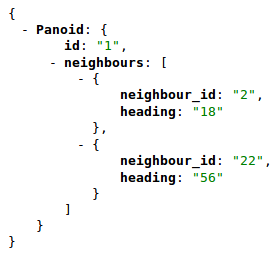
\includegraphics[width=0.4\textwidth]{ScreenshotAPIBeispiel.png}
\caption[API Beispiel]{Bildschirmfoto des gegebenen API Beispiels}
\label{fig:ScreenshotAPIBeispiel}
\end{figure}

Die Darstellung dieser Ausgabe wurde mit Hilfe eines Darstellungstools zur besseren Lesbarkeit optimiert. Im Normalfall würde die Ausgabe in einer Zeile dargestellt werden. Daran ist wiederrum zu sehen, dass das Ausgabeformat nicht auf menschliche Lesbarkeit ausgelegt ist.

Nachdem das ausgebende System der Beispielschnittstelle implementiert wurde, wird dieses im Folgenden angefragt und ausgewertet. Die Anfragen erfolgen, wie bereits erwähnt, asynchron innerhalb einer Javascript-Funktion. Asynchron bedeutet dabei, dass die Anfrage unabhängig von dem Aufbau der restlichen Seite ausgeführt wird. Während die Seite lädt und zum Beispiel HTML darstellt o.ä. wird unabhängig davon eine weitere Anfrage ausgeführt und aufbauend auf dem Ergbenis die Seite verändert.
In \verweis{Prototyp} wurde bereits die Funktion "`createCustomLink"' aus dem Anhang ~\ref{sec:AnhangJavascriptPrototyp} vorgestellt. In dieser Funktionen werden die sogenannten Links gesetzt, die letzen Endes die Navigationspfeile abbilden. Im \verweis{Prototyp} wurden diese Links statisch gesetzt, im Folgenden sollen diese durch Aufrufen der API dynmaisch gesetzt werden. Dazu wird die Funktion \textit{createCustomLink} zunächst um einen Funktionausruf der Funktion "`getPanoJson"' erweitert. Diese Funktion ist dafür zuständig die oben definierte API mit einer übergebenen ID anzufragen und ein JSON-Objekt an die aufrufende Methode zurückzuliefern. Die Implementierung dieser Funktion wird in folgender \listing{Dynamisch Nachbarn nachladen} gezeigt:

\lstinputlisting[language=JavaScript,caption={Dynamisch Nachbarn nachladen},label={lst:Dynamisch Nachbarn nachladen}]{Listings/Dynamisch_Nachbarn_nachladen.js}

Die Funktion \textit{getPanoJson} wird in Zeile 5 aufgerufen und fragt dann über einen sogenannten \textit{XMLHttpRequest} die oben definierte URL an (Zeile 25). Da die Antwort eine unformartiertes Textdokument ist (es ist nicht möglich über HTTP Objekte zu übertragen) muss dieser in ein JSON-Objekt umgewandelt werden, man spricht dabei von "`parsen"' (Zeile 28). Die Elemente des zurückgelieferten JSON-Objektes (Zeile 30) können danach von der aufrufenden Funktion referenziert werden. Über "`pano.neighbours"' (Zeile 7) erhält man beispielsweise eine Liste aller Nachbarn, die im oben dargestellten Quellcode durchlaufen und in die \textit{Links}-Liste geschrieben werden (Zeile 8ff.). Durch den einfachen Aufruf von Elementen eines Objektes zeichnet sich an dieser Stelle die oben angesprochene Objektorientierung besonders aus.

Der Prototyp wird durch diese Implementierung dynamisch und stellt die Informationen dar, die im Administrationsbereich
gepflegt wurden.

An dieser Stelle des Entwicklungsprozesses ist der Administrationsbereich vollständig funktional abgebildet und die Benutzeransicht greift über APIs auf die hinterlegten Informationen zu. Die Umsetzung des Projektes ist damit abgeschlossen.